\chapter{Dostupnost a distribuce PROTOPlantu}
Jak popisuji v~úvodu, jedním z~cílů, který jsem si dal na začátku práce na PROTOPlantu bylo šíření pod licencí open-source.
Toto jsem dodržel. 
Celý software PROTOPlantu je šířen pod licencí MIT, ostatní části (Hardware, atd.) včetně textu této práce je poté pod CC BY-NC-SA 4.0.
Co se týče hardwaru, převzatý hardware (senzory, procesor a další moduly) je z~licence vyňat.
Člověk, který tedy elektrotechnice a programování rozumí si poté může PROTOPlant bez problému sestavit sám v~pohodlí domova.

Ovšem stále je obrovské množství lidí, kteří na sestavení PROTOPlantu nemusí mít dostatečné znalosti, nebo nemají čas si jej sestavovat.
Z~toho důvodu plánuji zahájit výrobu a distribuci mého systému jakožto hotových komponent, které stačí nainstalovat a zapojit.
Ke dni \It{20. 2. 2020} jsem ve fázi, kdy připravuji výrobní podklady jednotlivých komponent, a provádím kroky vedoucí k~založení podniku.
Již v~minulém roce jsem provedl průzkum, který ukázal, že o~PROTOPlant by skutečně byl zájem.

\section{Případové studie}
Pro názorný příklad použití PROTOPlantu uvádím konkrétní případové studie.

\subsection{Malý skleník s užitkovými rostlinami}
Zahrádkář pěstující plodiny čistě pro zásobování sebe a své rodiny čerstvou zeleninou vlastní skleník s plochou obdělávané půdy 6x3 metry.
Výška skleníku jsou přibližně dva metry, jeho objem je tedy vzhledem k tvaru skleníku \B{menší, než 36~m\superscript{3}}.
Pro dostatečné pokrytí prostoru senzorikou tedy stačí dva senzory teploty (viz kapitola \ref{sec:DS18B20}) a dva senzory vzdušné vlhkosti (viz kapitola \ref{sec:DHT22}). 
Vzhledem k obdělávané ploše, stačí použít 4 senzory půdní vlhkosti.
Zavlažování je vzhledem k pěstovaným rostlinám řešeno děrovanou hadicí položenou přímo na půdě.

\fxnote[author=PŠ]{Zde přibudou fotografie babiččina skleníku a tabulka s cenami (dnes večer to spočítám)}

\subsection{Středně velký skleník s okrasnými rostlinami}
Skleník, ve kterém PROTOPlant průběžně testuji je určen pro pěstování orchidejí. 
Jeho plocha je přibližně 10~x~4~m.
Většina rostlin je v květináčích s molitanem či substrátem zavěšena v prostoru, nebo položena na stole.
Teplotní senzory jsou zde použity 4, senzory vlhkosti 3.
Vzhledem k tomu, že většina z těchto rostlin je epifytní, nesnášejí trvale vlhkou půdu. 
Z tohoto důvodu je zavlažování řešeno rozprašovačem umístěným pod stropem skleníku a upraveným nastavením jeho spínání.
Neprobíhá tedy tak často.

\fxnote[author=PŠ]{Zde přibude tabulka s cenou}

\begin{figure}[htbp]
    \centering
    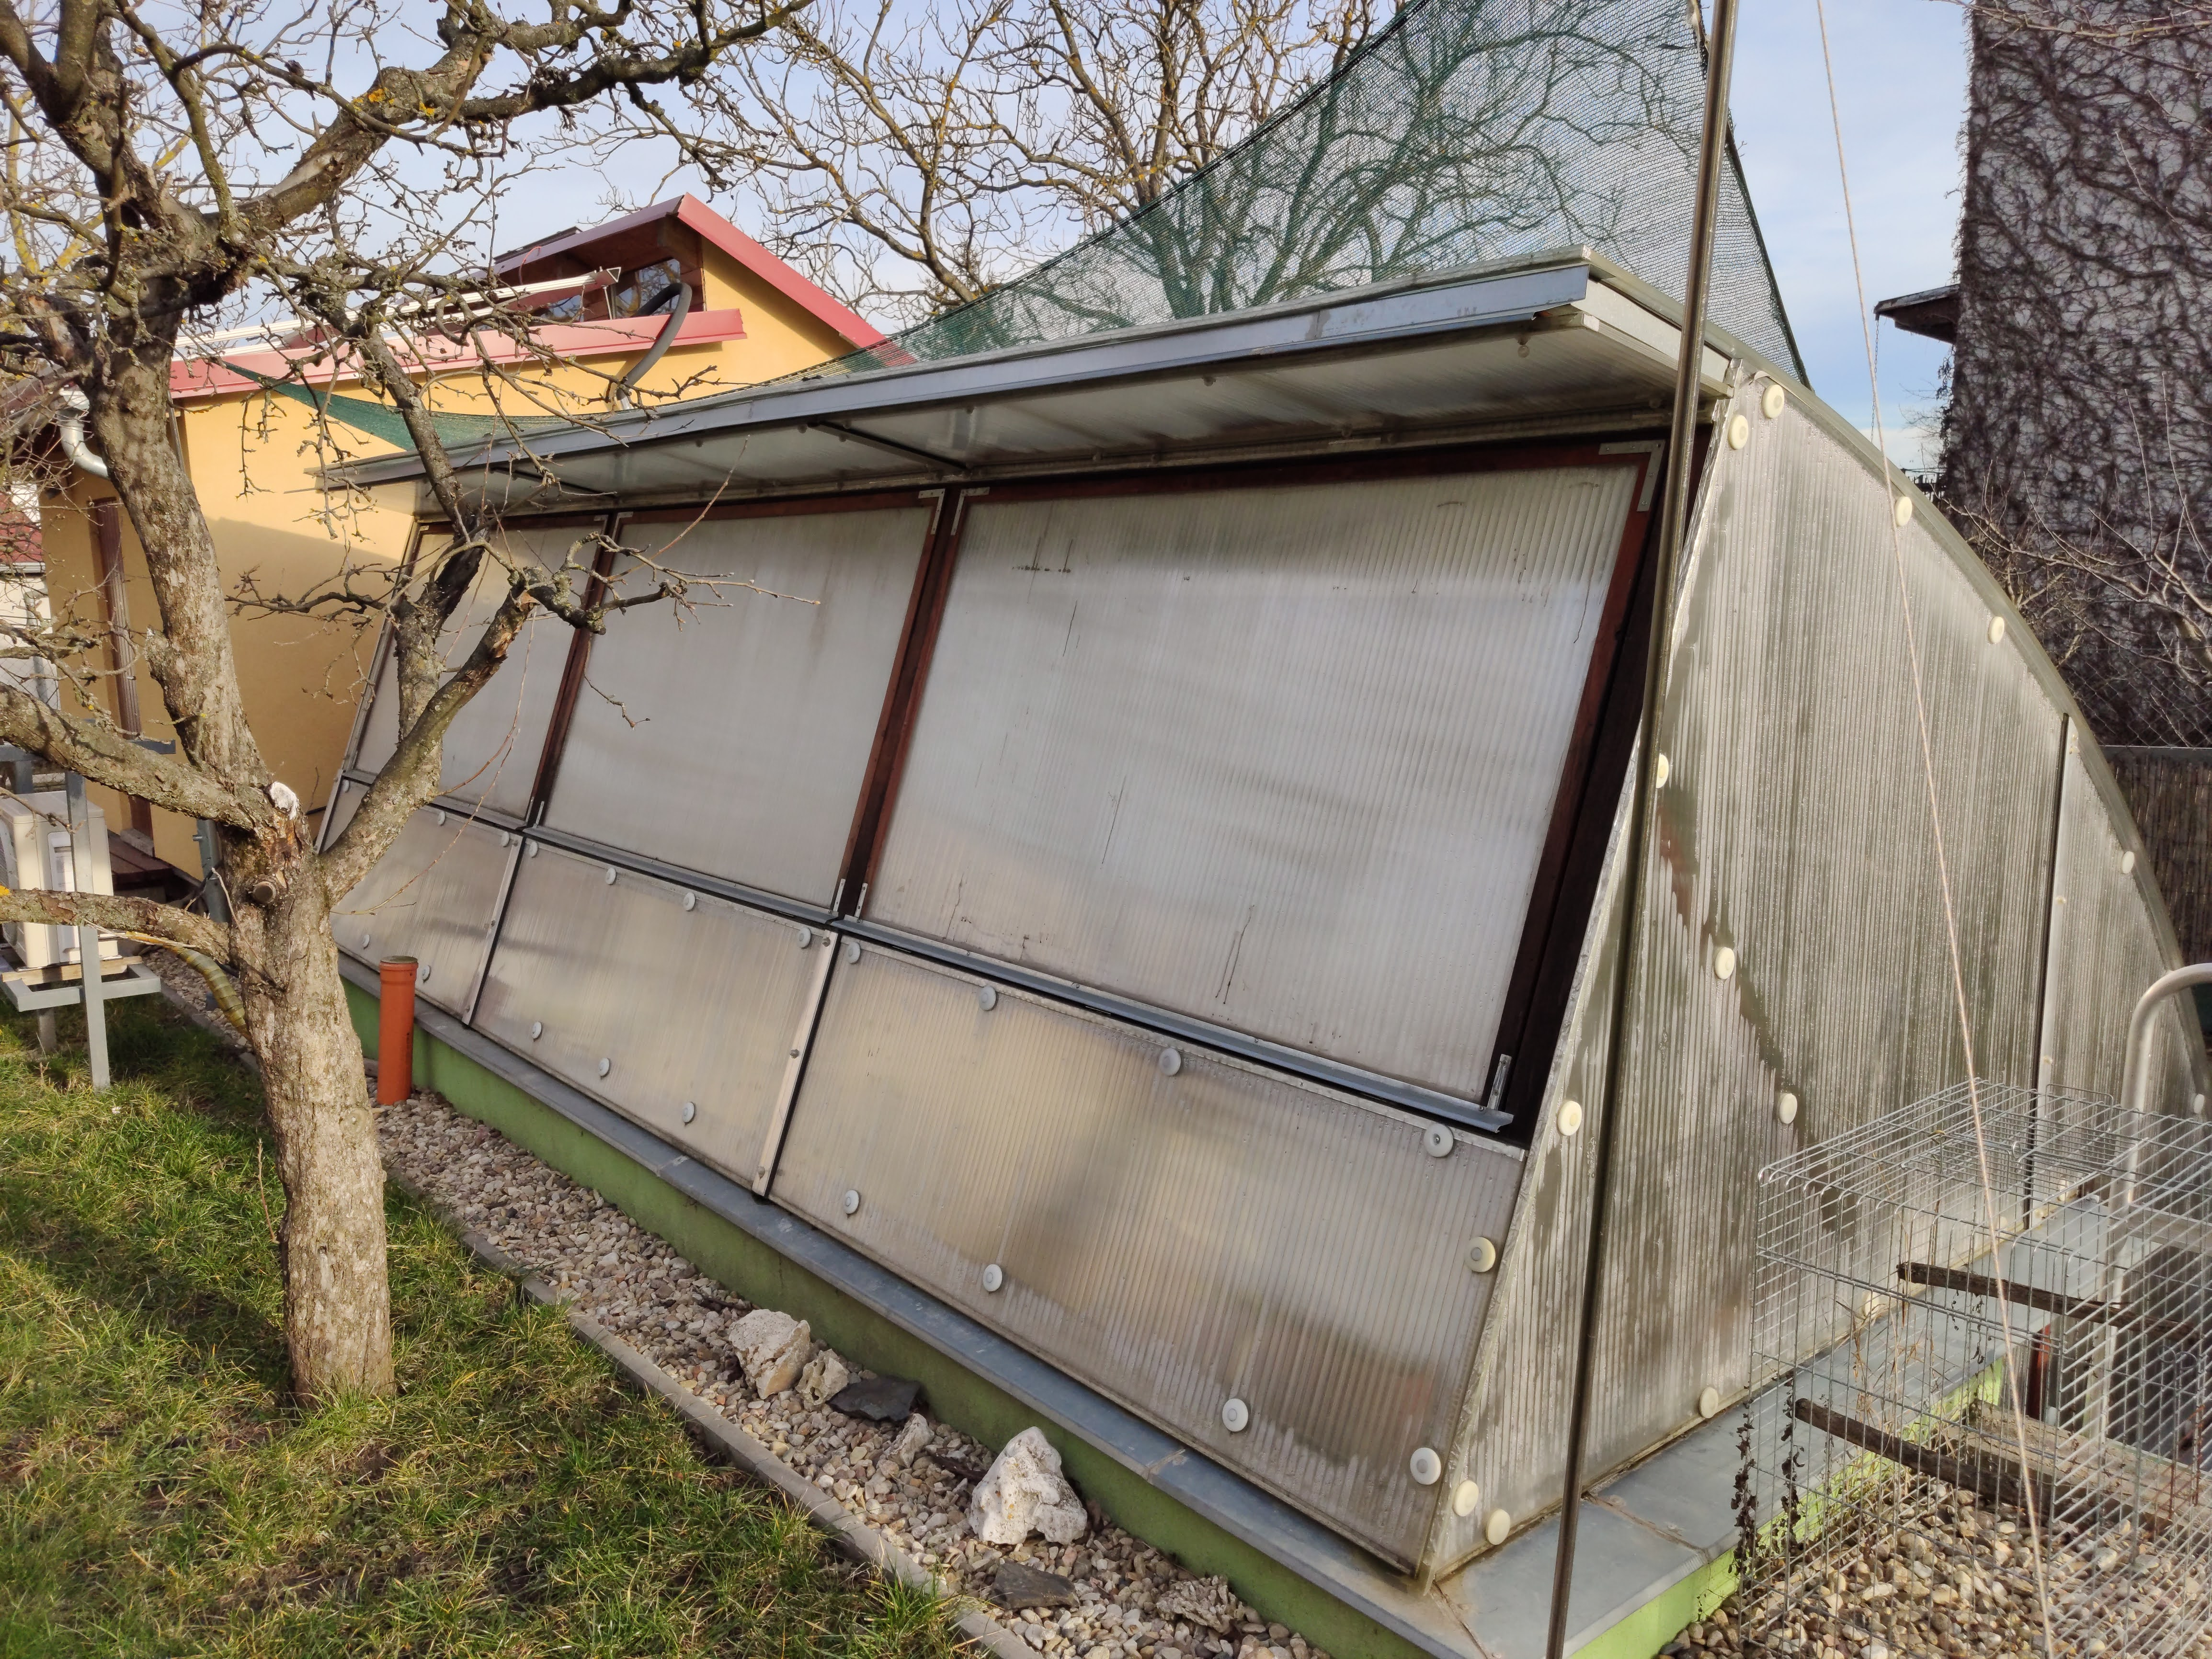
\includegraphics[width=\textwidth]{img/PHOTOS/OrchidHouse_EXTERIOR.jpg}
    \caption{Exteriér testovacího skleníku}
    \label{fig:OrchidHouse_EXTERIOR}
\end{figure}

\begin{figure}[htbp]
    \centering
    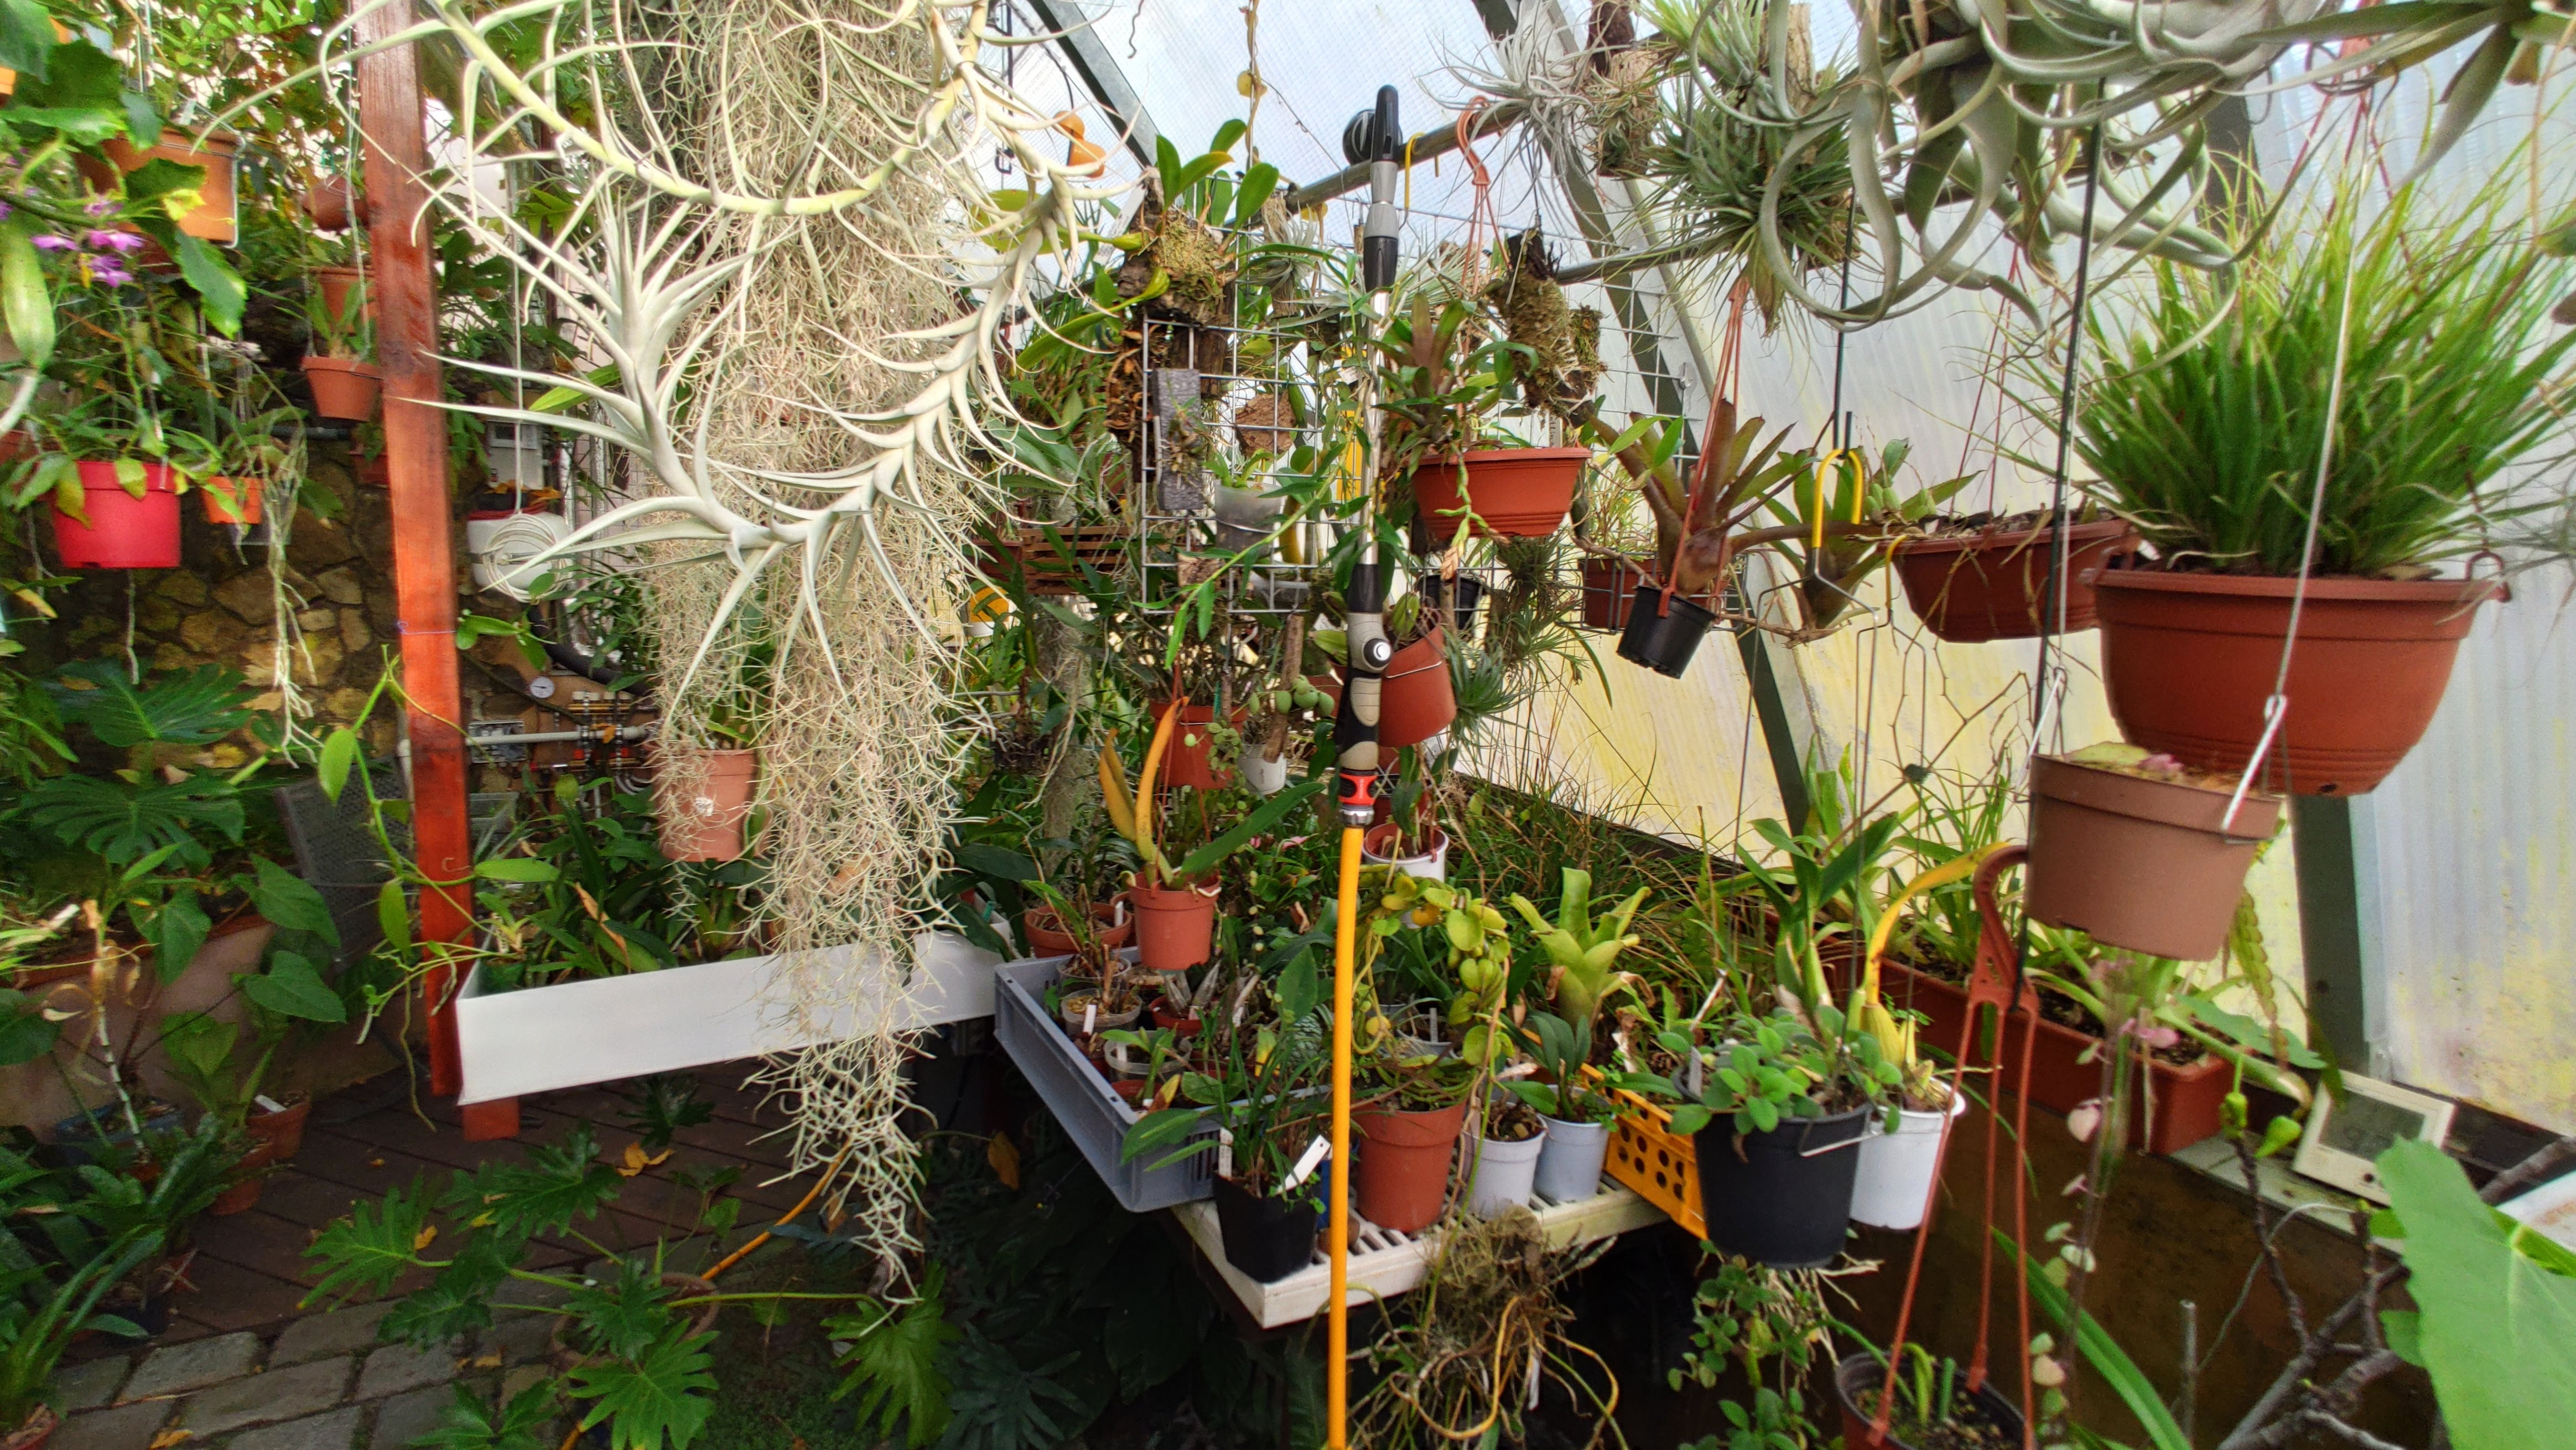
\includegraphics[width=\textwidth]{img/PHOTOS/OrchidHouse_INTERIOR.jpg}
    \caption{Interiér testovacího skleníku}
    \label{fig:OrchidHouse_INTERIORs}
\end{figure}
\newpage